\chapter{Design Details}

\label{sec:design_details}

This chapter details the technical approach to solving the design problem, presenting the system architecture and its decomposition into subsystems, each of which is elaborated in the subsequent chapters.

\section{Solution Statement}

The solution is a single 4-axis gantry robot operating under the human--robot collaboration paradigm established in Section~\ref{sec:operational_paradigm}, which handles the heavy lifting of the process while workers retain the dexterous tasks. The X and Y axes are belt-driven, the Z-axis is rack-and-pinion driven, and the yaw axis is directly driven, all by AC servo motors. The end-effector is purely vacuum-based, with suction cups and pressure feedback, and tracking of microwaves and boxes is through computer vision. All components are procured through local suppliers, with the control architecture built on open-source software to eliminate dependence on foreign proprietary expertise for programming and maintenance.

The primary ethical driver of the project is to address occupational safety in the factory; however, to retain the employment of line workers, the approach adopts human-robot collaboration. To promote sustainability, the project utilizes motors with the minimum sufficient power ratings and S-curve motion profiles to minimize energy usage. The automated handling of microwaves also targets waste reduction, as fewer microwaves are discarded due to manual lifting errors stemming from fatigue.

\section{Solution Overview}

Figure~\ref{fig:system_diagram} presents the overall system block diagram showing the flow of data, power, and mechanical motion across the system.

% TODO (Fix 3.4): Redraw this diagram with the following changes:
%   1. Make UART/USB arrow bidirectional
%   2. Group gearboxes with motors into single boxes
%   3. Label arrows with data types (e.g., "position commands", 
%      "sensor feedback") rather than protocols/voltages.
%      Put protocols in the chapter text, not the diagram.
\begin{figure}[H]
    \centering
    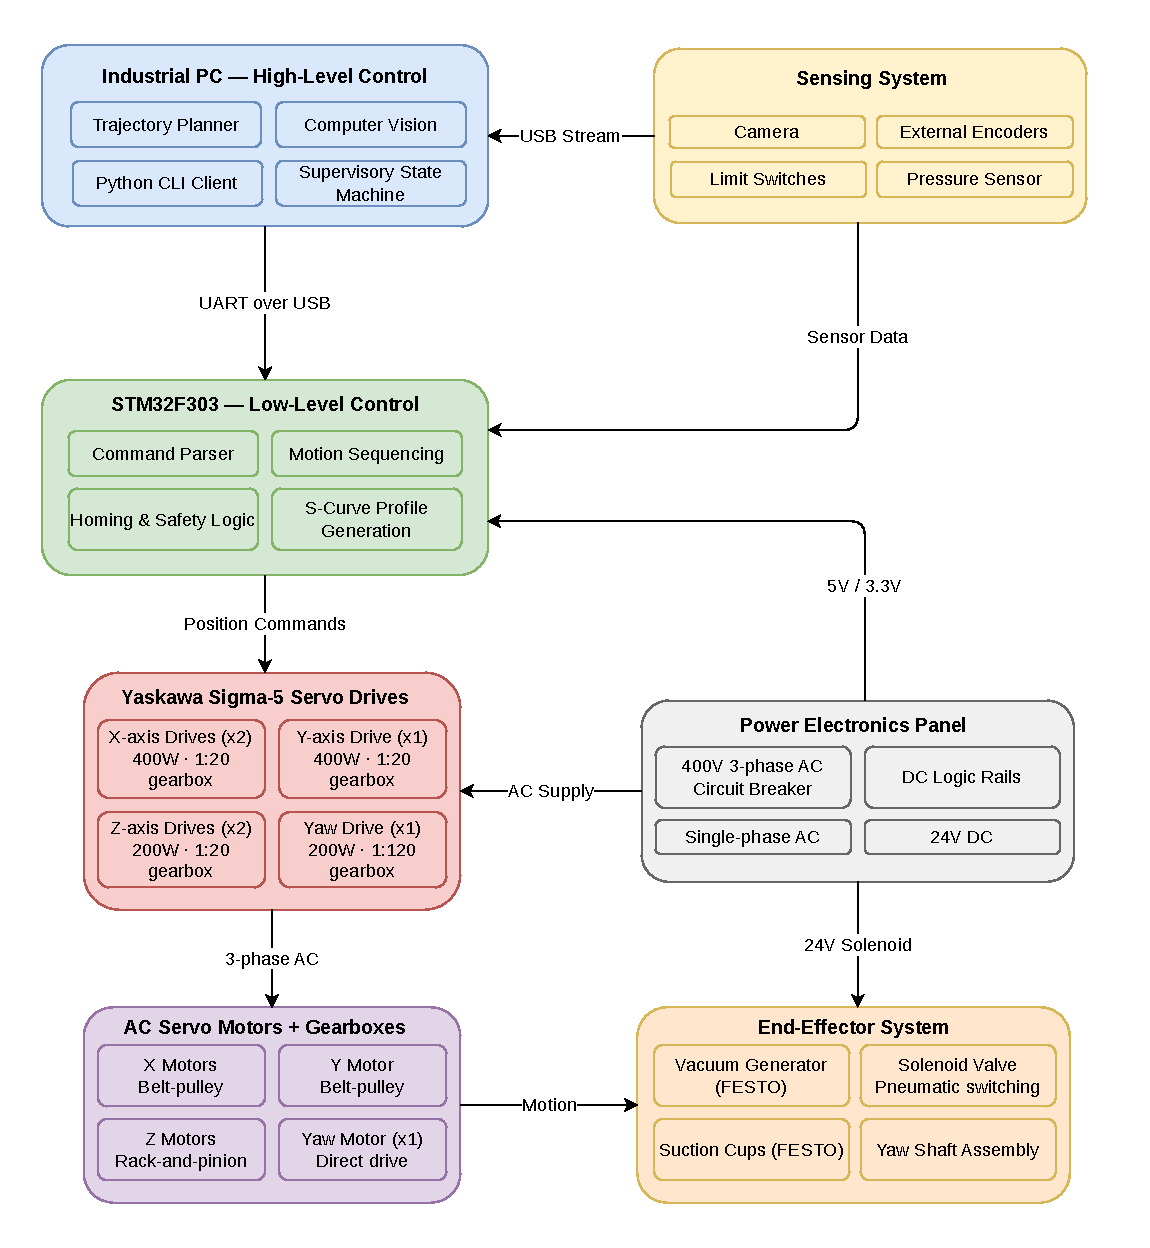
\includegraphics[width=\linewidth]{system_diagram.pdf}
    \caption{Overall system block diagram.}
    \label{fig:system_diagram}
\end{figure}

The system is structured as a hierarchy of control layers. An industrial PC performs computer vision and trajectory planning, forwarding position commands to an STM32F303 microcontroller over UART. The microcontroller generates S-curve motion profiles and issues pulse/direction signals to Yaskawa Sigma-5 servo drives, which perform closed-loop position control of the AC servo motors. The motors drive the mechanical axes through belt-and-pulley (X, Y), rack-and-pinion (Z), and harmonic drive (yaw) transmissions. A vacuum-based end-effector with solenoid-controlled switching handles the payload, while a sensing system comprising a global shutter camera, limit switches, external encoders, and a pressure sensor closes the feedback loop. The power electronics panel distributes factory 400V three-phase AC to the drives and generates the 24V DC and logic-level rails required by the remaining subsystems. Each of these subsystems is detailed in Chapters~4 through~11.


\section{System Details}

While the block diagram demonstrates how the hardware is set up --- particularly how data, power, and mechanical translation flow across the system --- the logical subsystems manifest slightly differently. For example, the domain of the camera dwarfs that of the remaining sensors, and warrants an entire chapter. The mechanical structure is what multiple parts of the robot rely on, but is passive in terms of data flow, and cannot be represented easily in the diagram.

Hence, the project is partitioned into the following subsystems.

\begin{itemize}
    \item \textbf{Mechanical Structure (Chapter~4):} The frame contains two parallel X-axis beams, a Y-axis bridge spanning between them, a Z-axis mast hanging from the carriage, and an assembly incorporating both the yaw and the end-effector at the bottom. Linear bearings and guides bear the weight of the moving axes.
    \item \textbf{Drive Mechanisms (Chapter~5):} The X and Y-axes employ belt \& pulley systems, while the Z-axis is driven by a spur rack \& pinion mechanism. The yaw axis is directly driven through a high-ratio gearbox.
    \item \textbf{Motor Actuation (Chapter~6):} Yaskawa Sigma-5 AC servos provide closed-loop position control, each paired with planetary gearboxes sized to handle the payload inertia while meeting speed requirements.
    \item \textbf{Power Electronics (Chapter~7):} The electrical subsystem partitions the factory 400V three-phase supply into drive power, single-phase logic supply, 24V DC for brakes and solenoids, and 5V/3.3V logic rails.
    \item \textbf{End-Effector (Chapter~8):} A vacuum-based lifting mechanism using six suction cups (two large, four small) with a yaw axis consisting of a motor coupled via a shaft and angular contact bearings.
    \item \textbf{Low-Level Control (Chapter~9):} The STM32F303 interfaces with the Yaskawa drives via a differential pulse/direction protocol, generates S-curve motion profiles, and implements homing routines using limit switches.
    \item \textbf{Computer Vision (Chapter~10):} An AR0234 global shutter camera feeds a detection and pose estimation pipeline to provide the X, Y, and yaw coordinates needed for alignment.
    \item \textbf{High-Level Control (Chapter~11):} A supervisory layer on the industrial PC communicates with the STM32 via UART over USB, providing teleoperation, trajectory planning, and state machine logic.
\end{itemize}

Each of the subsystems is explained in the following chapters.